\chapter{Model Architecture and Training}

\section{YOLOv8 Architecture}

YOLOv8 (You Only Look Once, version 8) is a single-stage object detection framework developed by Ultralytics. Unlike two-stage detectors such as Faster R-CNN, YOLOv8 performs detection in a single forward pass of the network, enabling real-time inference speeds. The architecture comprises three principal components: a backbone for feature extraction, a Feature Pyramid Network (FPN) neck for multi-scale feature aggregation, and an anchor-free detection head.

The backbone employs Cross-Stage Partial bottleneck blocks with two convolutions (C2f), which improve gradient flow and reduce computational redundancy compared to earlier YOLO versions. The FPN neck fuses feature maps from multiple backbone stages, allowing the model to detect objects at different scales simultaneously --- a critical property for this task where traffic lights range from Tiny to Small in size. The detection head operates at three spatial scales, producing predictions for small, medium, and large objects independently.

Figure~\ref{fig:arch} presents the architectural block diagram of YOLOv8s.

\begin{figure}[ht]
    \begin{center}
        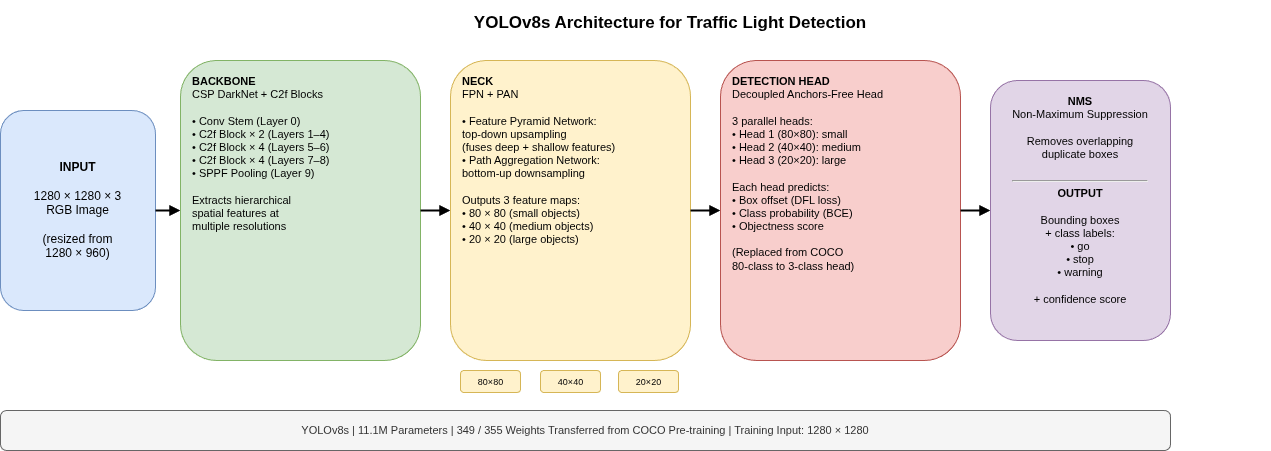
\includegraphics[width=\textwidth]{Images/Diagrams/yolov8_arch.png}
    \end{center}
    \caption{Block diagram of the YOLOv8s architecture showing the C2f backbone, FPN neck, and multi-scale detection head.}
    \label{fig:arch}
\end{figure}

\section{Model Selection Rationale}

The YOLOv8 family offers multiple size variants: nano (YOLOv8n, 3.2M parameters), small (YOLOv8s, 11.1M parameters), medium (YOLOv8m, 25.9M parameters), large (YOLOv8l), and extra-large (YOLOv8x). The selection of YOLOv8s was motivated by the bounding box size analysis presented in Section~2.3.2: as 96\% of traffic light instances in the dataset are classified as Tiny or Small, detecting such objects requires a deeper feature pyramid with richer low-level spatial information. YOLOv8n, despite being faster, has a shallower backbone insufficient for resolving fine-grained features at these scales. YOLOv8s provides an optimal balance between detection capability for small objects and training efficiency on available hardware.

\section{Transfer Learning}

Transfer learning was employed to initialise the model with weights pre-trained on the COCO dataset (Common Objects in Context), which contains 80 object categories and over 330,000 images. This pre-training endows the backbone with learned representations of low-level visual features such as edges, textures, and colour gradients --- features that are directly applicable to traffic light detection.

During fine-tuning, 349 of the 355 weight parameter groups were transferred from the COCO-pretrained checkpoint. The six remaining groups, corresponding to the final detection head output layers, were reinitialised to accommodate the three-class output space (go, stop, warning) in place of the original 80-class space. This strategy substantially reduces the data and computation required to achieve high accuracy compared to training from random initialisation.

\section{Training Configuration}

Table~\ref{tb:config} summarises the key hyperparameters used during training.

\begin{table}[htbp]
\caption{Training configuration and hyperparameters.}
\label{tb:config}
\centering
\small
\begin{tabular}{>{\raggedright\arraybackslash}p{0.32\textwidth} >{\raggedright\arraybackslash}p{0.20\textwidth} >{\raggedright\arraybackslash}p{0.38\textwidth}}
\toprule
\textbf{Parameter} & \textbf{Value} & \textbf{Rationale} \\
\midrule
Input resolution (imgsz) & 1280\,px & Preserves detail in small traffic lights \\
Batch size & 16 & Safe VRAM usage on RTX 5090 ($\sim$15\,GB) \\
Maximum epochs & 50 & Sufficient for convergence with early stopping \\
Early stopping patience & 20 & Halts training if no mAP improvement for 20 epochs \\
Mosaic augmentation & 1.0 & Combines 4 images; increases object density \\
Mixup augmentation & 0.1 & Blends image pairs; improves generalisation \\
Horizontal flip & 0.5 & Mirrors scenes; handles left/right light positions \\
Initial learning rate & 0.01 & Standard SGD starting point \\
Optimiser & SGD & Selected automatically by Ultralytics \\
AMP & Enabled & Halves VRAM usage via 16-bit arithmetic \\
GPU & RTX 5090 (32\,GB VRAM) & Supports large-resolution batches without out-of-memory errors \\
\bottomrule
\end{tabular}
\end{table}

\section{Training Process and Convergence}

\subsection{Loss Curves}

YOLOv8 optimises three loss components simultaneously during training. Box loss measures the accuracy of predicted bounding box coordinates. Classification loss measures the accuracy of class predictions. Distribution Focal Loss (DFL) refines the precision of box edge localisation. Figure~\ref{fig:curves} illustrates the evolution of all three loss components across training epochs for both the training and validation sets.

\begin{figure}[ht]
    \begin{center}
        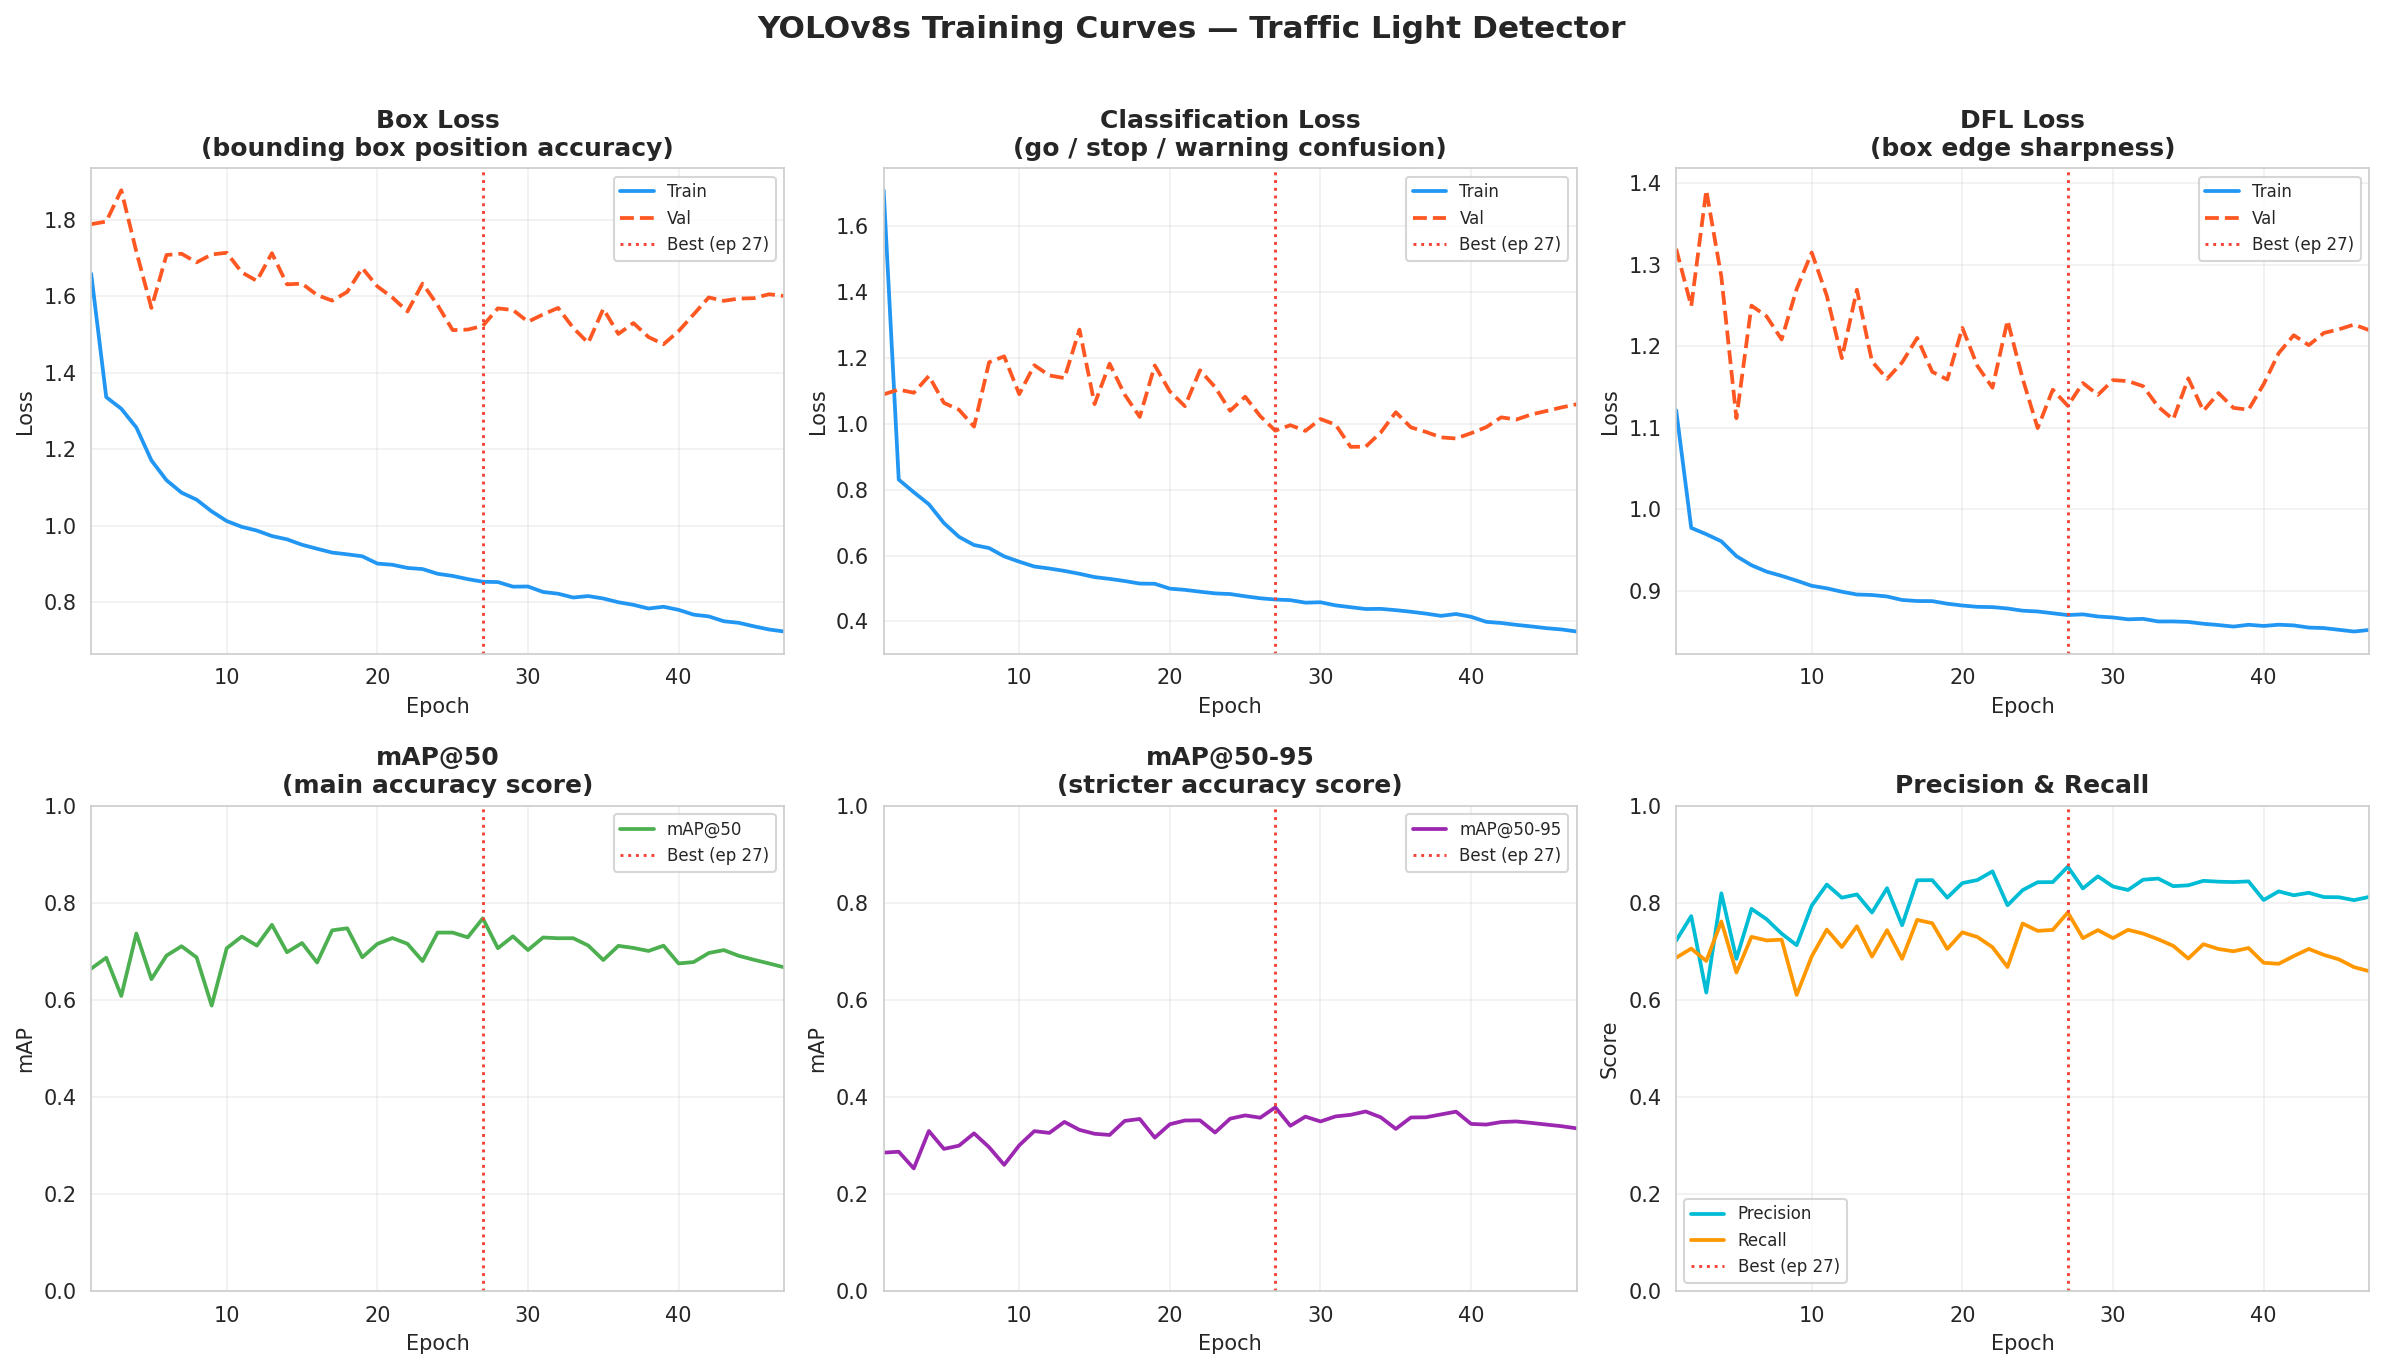
\includegraphics[width=\textwidth]{Images/Chapter3/training_curves.png}
    \end{center}
    \caption[Training and validation curves]{Training and validation loss curves (box loss, classification loss, DFL loss) alongside accuracy metrics (mAP@50, mAP@50-95, Precision, Recall) across 47 training epochs. The red dotted vertical line marks epoch 27, where the best model was saved.}
    \label{fig:curves}
\end{figure}

All three loss values decrease monotonically across training epochs, confirming that the model is learning effectively. The classification loss exhibits the most dramatic reduction, from 1.71 at epoch 1 to 0.37 at epoch 47, indicating that the model rapidly learned to distinguish between the three traffic light states. Early stopping was triggered at epoch 47, as no improvement in validation mAP@50 was observed for 20 consecutive epochs following the peak at epoch 27.

\subsection{Accuracy Progression}

The validation mAP@50 improved from 0.664 at epoch 1 to a peak of 0.768 at epoch 27. Following this peak, the metric plateaued and exhibited minor oscillations without further improvement, indicating that the model had reached its representational limit under the current training configuration. The best model weights (best.pt) were automatically saved at epoch 27. Total training time was approximately 2 hours and 14 minutes on an NVIDIA GeForce RTX 5090 Graphics Processing Unit (GPU).

\subsection{Precision and Recall Trends}

Throughout training, precision reached 0.874 while recall achieved 0.780 at the best epoch. The higher precision relative to recall indicates that the model is conservative in its detections --- when it identifies a traffic light, it is correct with high probability (87.4\%), but it misses approximately 22\% of actual traffic lights in the scene. This behaviour is consistent with the model's difficulty in detecting the smallest instances and the underrepresented go class.

%%%%%%%%%%%%%%%%%%%%%%%%%%%%%%%%%%%%%%%%%%%%%%%%%%%%%%%%%%%%%%%%%%%%%%%%%%%%%%%%%%%%%%%%%%%%%%%%%%
%%% END OF FILE
%%%%%%%%%%%%%%%%%%%%%%%%%%%%%%%%%%%%%%%%%%%%%%%%%%%%%%%%%%%%%%%%%%%%%%%%%%%%%%%%%%%%%%%%%%%%%%%%%%
